\section{Apparatus}
\label{section:apparatus}
This section describebd the 

\subsection{Microsoft Azure Kinect description}

 Microsoft Azure Kinect\footnote{Official website: \url{https://azure.microsoft.com/en-us/services/kinect-dk/}} cameras are used to capture the data in order to render the scene in 3D. The Azure Kinect camera is composed of several sensors, see figure \ref{figure:kinect_sensors}. The 1 megapixel depth sensor and the 12 megapixel RGB sensor are  used for the experiment to render the scene in 3D. Accelerometer and gyroscope with IMU and a 7 microphone array could be used for other purposes. The external sync pin makes it easier to synchronise sensors streams from multiple Kinect cameras.
 
\begin{figure}[H]
    \centering
    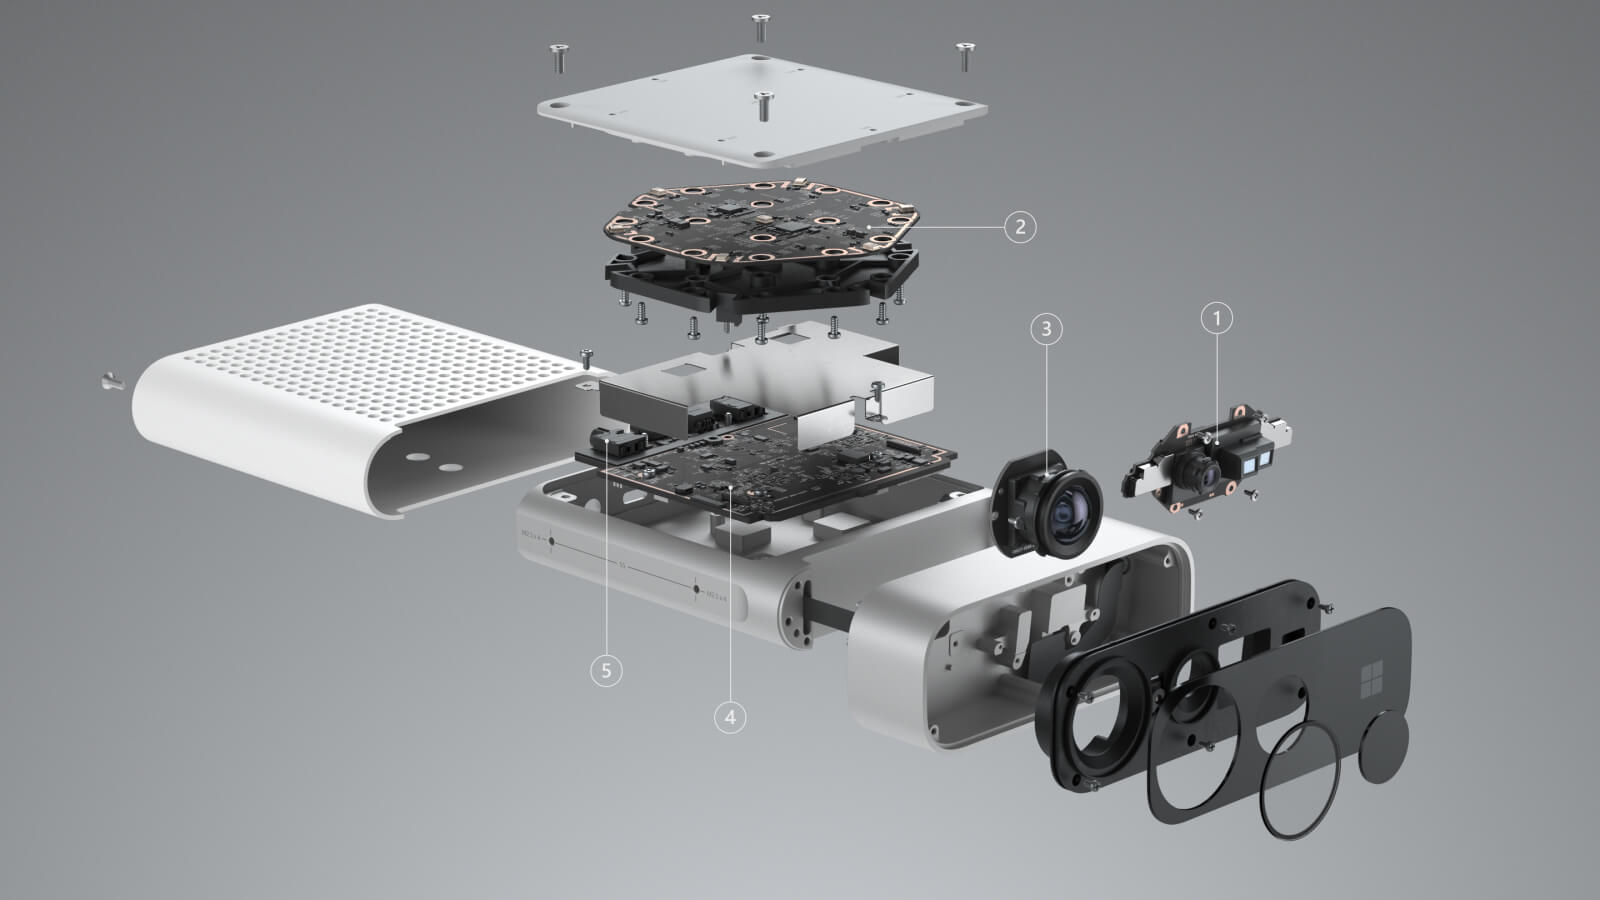
\includegraphics[width=0.65\textwidth]{images/apparatus/kinect_sensors.jpg}
    \caption{Microsoft Azure Kinect camera. 1) 1-MP depth sensor 2) 7-microphone array 3) 12-MP RGB video camera 4) Accelerometer and gyroscope (IMU) 5) External sync pins to easily synchronize sensor streams from multiple Kinect devices. Source: \cite{noauthor_azure_nodate}}
    \label{figure:kinect_sensors}
\end{figure}

\subsection{Depth sensor: Time of flight}
% https://docs.microsoft.com/fr-fr/azure/Kinect-dk/depth-camera

\subsubsection{Operating principle}

The Azure Kinect depth camera implement the Amplitude Modulated Continuous Wave (AMCW) Time-of-Flight (ToF) principle. A modulated illumination in the near-infrared (NIR) spectrum is casted onto the scene. Then an indirect measurement of the time it takes for the light to travel from the camera to the scene and back is recorded. These measurements generates a depth map which is a set of Z-coordinate values for every pixel of the image. The unit of the depth map is the millimetre. Figure \ref{figure:depth_sample} shows an example depth image. Invalid depth pixels are in black colour outside the hexagon.

\begin{figure}[H]
    \centering
    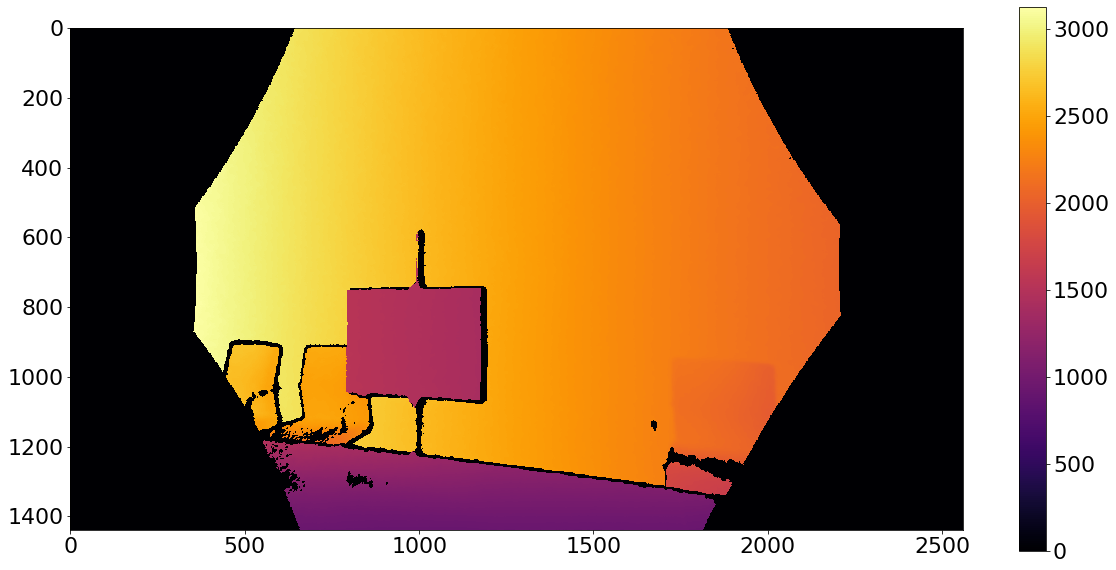
\includegraphics[width=0.65\textwidth]{images/depth_sample.png}
    \caption{Depth image of a scene. Narrow filed of view mode. Black pixel outside the hexagon represents invalid depth information. The scale is in millimetre.}
    \label{figure:depth_sample}
\end{figure}

\subsection{3D coordinate system}
\label{section:3D coordinate system}

%  Each sensor is associated with its own coordinate system. 

Figure \ref{figure:coordinate-systems-camera-features} presents the 3D coordinate system of the Microsoft Azure Kinect camera. [X,Y,Z]-coordinate triplets with units in millimetres represent points in the 3D coordinate system. The focal point of the camera is also the origin [0,0,0]. The positive X-axis points right, the positive Y-axis points down and the positive Z-axis points forward.The depth camera is tilted 6 degrees downwards of the colour camera. This coordinate system is used for the rest of the thesis.

\begin{figure}[H]
    \centering
    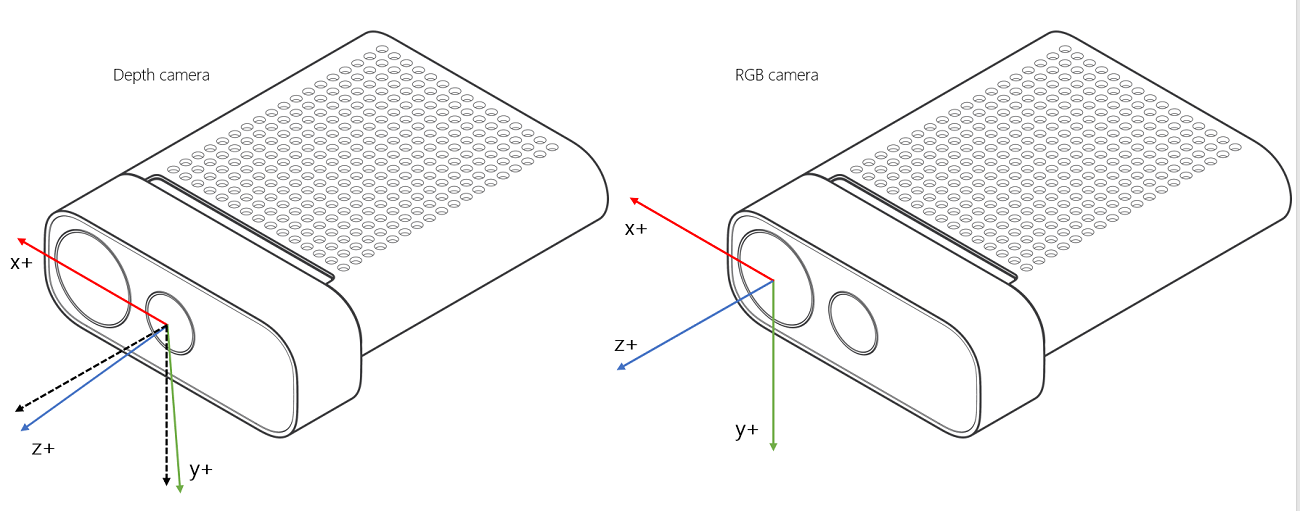
\includegraphics[width=0.65\textwidth]{images/apparatus/coordinate-systems-camera-features.png}
    \caption{3D coordinate system of the Microsoft Azure Kinect camera}
    \label{figure:coordinate-systems-camera-features}
\end{figure}

% \subsubsection{Depth sensor performance}

% \subsubsection{Systematic Error}

% \subsubsection{Random error}

% \subsection{Invalidation}